\documentclass[9pt]{article}
%Gummi|065|=)

\usepackage{amsmath}
\usepackage{amsfonts} 
\usepackage{hyperref}
\usepackage{color}
\usepackage{graphicx}
\usepackage{float}

\usepackage[most]{tcolorbox}
\textheight = 20 cm

\renewenvironment{abstract}
 {\small
  \begin{center}
  \bfseries \abstractname\vspace{-.5em}\vspace{0pt}
  \end{center}
  \list{}{
    \setlength{\leftmargin}{.9cm}%
    \setlength{\rightmargin}{\leftmargin}%
  }%
  \item\relax}
 {\endlist}
 
\begin{document}
\title{\textbf{AuditOcean,\\a platform for decentralized auditing: Descentralization level }}
\author{Juan C. Rey\\ \emph{Smart Contract Audit Token}\footnote{Smart Contract Audit Token (SCAT). Website: \url{www.scatdao.com} This work is supported by SCAT team.}\\}
\date{May 30, 2023}

\maketitle

\renewcommand*\abstractname{\textbf{}\hfill}

\abstract{
\textbf{Abstract.} This chapter aims to describe the transitionable features of AuditOcean platform for decentralized audits. The transitionable features are those centralized functional requirements that the platform needs to perform the audits and that could be replaced with decentralized alternatives using a smart contract on the Cardano network.
}

\section{Introduction}
By using a decentralized audit system it is possible to eliminate potential corruption points that may exist in a centralized audit system such as the choice of auditors or the interest of third parties to influence the outcome of an audit report. AuditOcean is a blockchain community space designed for research and project auditing. The community decides through its voting power which projects should be audited. Users can add the projects they want through the public repository https://dyortool.io/. Once the user adds a project a dedicated page is created where users can select it as a project to be audited in the active audit round. The main product is to make fundamental analysis reports (advanced research questions outline) and soon formal verification reports and technical testing reports to cardano smart contracts.

\section{ Transitional Features }
The transitional features are all functional requirements necessary to perform an audit round that could be replaced with decentralized alternatives using a smart contract on the Cardano network. Governance, audit round administration, assignment of auditors and report minting are the most important. 


\subsection { Round administration }

An audit round is a synchronous four-stage process and its purpose is to conduct audits of projects chosen by the community. Each audit round has a unique name or index characterized by having the letter R + a consecutive number, e.g. \emph{R5, R7, R10}. 

\begin{figure}[ht]
  \centering
  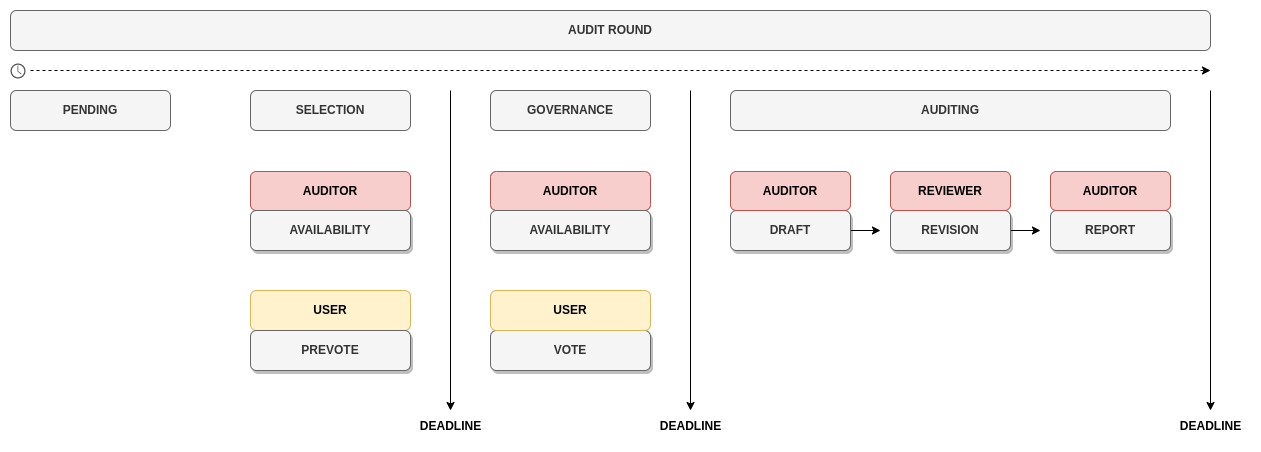
\includegraphics[width=0.86\textwidth]{round.png}
  \caption{Audit round}
  \label{fig:mi_imagen}
\end{figure}

When an audit round is created the administrator can start its stages synchronously by executing an endpoint on the backed with the desired parameters. The \emph{service-audits} pod receives the http request and sends an event to the \emph{Bull-MQ} queuing system which controls when a stage finishes according to the assigned time.

\begin{figure}[ht]
  \centering
  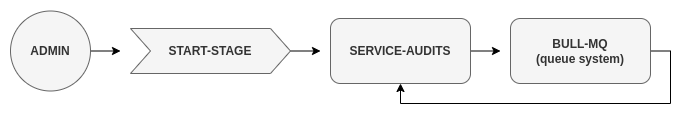
\includegraphics[width=0.86\textwidth]{admin.png}
  \caption{Stage administration}
  \label{fig:mi_imagen}
\end{figure}

In this centralized configuration the administrator and the queuing system control the states of the active audit round. The states of an audit round are the \emph{Pending}, \emph{Selection}, \emph{Governance}, and \emph{Auditing} stages. Each of these states transitions synchronously, that is, a stage cannot start if the previous stage has not finished, the transitions are sequential not parallel.

In computer science the concepts of state and machine of states are common. A state machine it is a mathematical model to describe the behavior of the different states of a system and their transitions based on conditions, events or triggers. Each state in a state machine represents a specific configuration of the system. It has an initial state that can transition to other states following the rules of the system. Each state within a state machine can execute actions, change variables and produce outputs according to the conditions specifically established for it. There are two types of state machines, the deterministic ones that for a given combination of state and input there is only one possible transition to the next state. And the non-deterministic ones that there can be multiple possible transitions from a given state for a particular input.

\begin{figure}[ht]
  \centering
  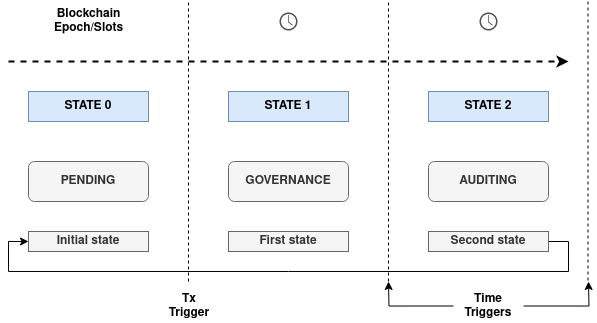
\includegraphics[width=0.9\textwidth]{machine.png}
  \caption{Round states}
  \label{fig:Round states}
\end{figure}

Figure 5 shows the deterministic state machine concepts applied to the stages of an audit round. The initial stage is a passive state that does not execute any logic necessary for the audit round. In order for the initial state to transition to the first state a trigger is needed. In this case, the DAO operational wallet interacts with a smart contract endpoint. For example, \emph{startRound} is the endpoint designed to start an audit round and receives the necessary parameters so that a round can start. Contracts in Cardano's EUTXO model need at least one initial transaction to trigger their design logic and configure its initial state.
\\
\\
\begin{tabular}{lr}
\textbf{initialStateMachine} \emph{:: MachineDatum}\\
\textbf{initialStateMachine}  = MachineDatum  \textbraceleft{}
\\ \hspace{60mm}currentState = 0, 
\\ \hspace{60mm}currentLabel = ``pending",
\\ \hspace{60mm}governanceLabel = ``governance",
\\ \hspace{60mm}auditingLabel = ``auditing" ,
\\ \hspace{60mm}governanceDuration = 0,
\\ \hspace{60mm}auditingDuration = 0
\\\hspace{60mm}\textbraceright{} 
\end{tabular}
\\
\\

 \emph{initialStateMachine} represents the initial state of the smart contract variables. These variables will remain in the default state indefinitely until the DAO wallet interacts with the \emph{startRound} endpoint which initiates an audit round. This is the trigger that makes the contract transition to the first state, that is, the governance stage.
\\
\\
\begin{tabular}{lr}
\textbf{initialStateMachine} \emph{:: MachineDatum}\\
\textbf{initialStateMachine}  = MachineDatum  \textbraceleft{}
\\ \hspace{60mm}currentState = 1, 
\\ \hspace{60mm}currentLabel = ``governance",
\\ \hspace{60mm}governanceLabel = ``governance",
\\ \hspace{60mm}auditingLabel = ``auditing" ,
\\ \hspace{60mm}governanceDuration = 100,
\\ \hspace{60mm}auditingDuration = 100
\\\hspace{60mm}\textbraceright{} 
\end{tabular}
\\
\\
Once the DAO wallet has interacted with the \emph{startRound} endpoint the contract will transition to the first state by assigning the new parameters to the contract variables. The duration parameters represent the time measured in Slots on the blockchain. The Plutus.Contract module has functions for dealing with time such as waiting for a certain amount of Slots to pass before proceeding with the execution of the contract. It is commonly used when implementing time-based behaviors or waiting for a specific deadline to be reached. It is possible to create a time-based trigger to transition to the second state and also to transition to the initial state without the need for external intervention managed by the time Slots of the blockchain.

\subsection { Governance } 
During the \emph{Selection} stage AuditOcean users select the project they want by pressing a button on the UI. The list of projects as the final result of this selection stage is submitted to a poll in an external governance platform called the summon platform.

\begin{figure}[ht]
  \centering
  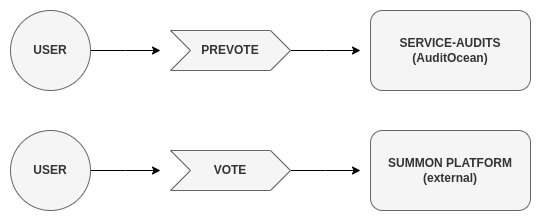
\includegraphics[width=0.6\textwidth]{votes.png}
  \caption{Selection and Governance stage
  }
  \label{fig:mi_imagen}
\end{figure}
This hybrid configuration (off-chain/on-chain) implies that the selection votes are created as documents within a centralized Mongo database. It is not possible for the community to directly audit the correct behavior of this process.

Once the selection stage is over, a poll is created on the summon platform where it is possible for the community to directly audit the transactions on the blockchain. The level of auditability of a decentralized governance system is not the same if there is a previous process that cannot be audited directly because it is carried out within private servers.

The way to get the best auditability is to remove the \emph{Selection} stage and have users vote with their wallets in the AuditOcean UI. It is not necessary to use an external service for governance, users will be able to log in from their wallets and vote for the project they want on the AuditOcean platform in a single stage.

\begin{figure}[ht]
  \centering
  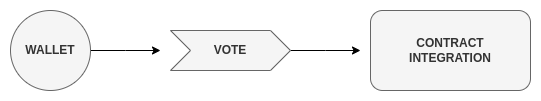
\includegraphics[width=0.6\textwidth]{last.png}
  \caption{Governance stage
  }
  \label{fig:mi_imagen}
\end{figure}



\subsubsection { State-Snapshot governance system } 


In the blockchain industry new projects are created daily and AuditOcean's list of projects will inevitably grow over time. It is possible for the community to add 1000 or 10000 projects if they wish. The consequence of this is the large number of indexes in the database. Managing such a number of indexes in a smart contract can be challenging because the limit of Kb per Tx is limited and it is not scalable. However, we can simplify the notion of long-length indices such as those used in databases by using consecutive natural numbers.

A 32-bit unsigned integer can be represented as 0 to 2147483647. A positive integer can be assigned as a unique index to each project added by the community in AuditOcean. In this way a smart contract could reference a large number of projects using only 32 Bits. For example, an user wants to vote for the project called SCATDAO which has the index 547 assigned, no other project has this index. The user connects their wallet containing the AUDIT utility token to the UI and performs the vote. The request goes to the backend and contract integration calling the endpoint \emph{ createVote } that receives a 32-bit positive integer as a parameter. The contract verifies if the parameter is valid and if the UTxO associated with that wallet address contain the AUDIT token. The contract finally checks if the index given as a parameter is less than or equal to \emph{projectIndex} variable of the contract which refer to the total number of projects that have been added to AuditOcean. If these conditions are correct the contract validates the Tx and adds a small mark in the metadata.


Once the governance stage is finished a snapshot is taken at the exact moment or Slot in which the stage ends. By making a query to the blockchain API it is possible to get the transactions associated with the address of the contract to validate the status of the transactions, verify if the transactions have been validated by the contract and verify the metadata of the transaction that provides the context resulting from the interaction with the contract. The metadata can help in identifying the purpose and status of the transaction. The information about the snapshot and governance stage is displayed in the platform UI for all users.

This configuration for the governance system guarantees speed, minimum computing time and the ability to validate millions of indexes using a simple condition:

\emph{ indexParam } $\in$ \emph{ projectIndex } $\Rightarrow$ \text{True}. 
 where \emph{ projectIndex } is the set of project indexes listed by the community. 

$\emph{ indexParam } \leq \emph{ projectIndex }$  $\Rightarrow$ \text{True}. where \emph{ projectIndex } is the total number of project indexes listed by the community.

\begin{figure}[ht]
  \centering
  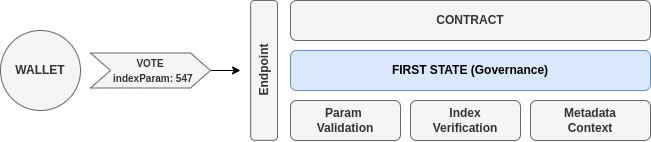
\includegraphics[width=0.85\textwidth]{vote.png}
  \caption{Governance
  }
  \label{fig:mi_imagen}
\end{figure}

The parameter \emph{ projectIndex } can be added by the DAO operational wallet when calling the \emph{startRound} endpoint. This parameter within the smart contract corresponds to a positive integer number. For example, in case there are 742 projects listed by the community, \emph{ projectIndex } will be 742. In the initial state of the contract this variable value is 0. At the end of the governance stage this variable will also be 0.

In the hypothetical case that the contract itself was designed to store the project indices in the form of assets or NFTs to later be consulted in the governance stage, this would add more logic to the contract and therefore computation time. For this reason it is a disadvantage to use the contract as a form of storage.

However, it is possible to assign a simple time-locked plutus script that allows to store the indices with project names in the form of small metadata using assets (1 asset per project) or simply stamping valid transactions without using assets. The DAO's operational wallet is the only one that will be able to interact with this plutus script. The address of the script on the blockchain will need to be included in the metadata when deploying the AuditOcean contract for the first time for auditability. This solution is scalable since multiple scripts can be used for this purpose. In this way there is complete audability with respect to the indices.


\begin{figure}[ht]
  \centering
  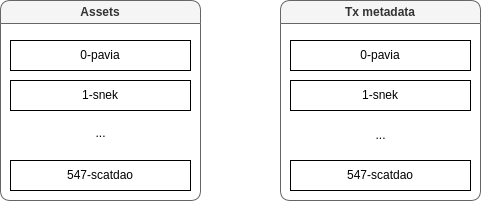
\includegraphics[width=0.822\textwidth]{indices.png}
  \caption{Index Auditability
  }
  \label{fig:mi_imagen}
\end{figure}

Another form of index auditability is public code repositories like Github or distributed storage systems like IFPS.
\subsection { Assignment of auditors }
   
The assignment of auditors to the projects to be audited can be a point of corruption if it is done centrally or by one person. For this reason, the best option is a decentralized assignment algorithm. There is not much complexity in the logic required for an equal assignment for all auditors. The main requirements are randomness and uniform distribution of the probability of being chosen as an auditor of a project. The Fisher-Yates algorithm ensures that each element has an equal probability of being placed in any position of the resulting permutation. This is useful since it can shuffle a finite list of indices. For example, A = [0, 50] where A is the list of indices from auditor 0 to auditor 50. Each index represent a specific auditor and they are ordered consecutively [0,1,2,3,4 .. 50]. When the algorithm is applied to the list the positions of the indices will change randomly. If AuditOcean needs 12 auditors for an audit round the first 12 indices from the shuffled list will be selected.\\

\emph {auditorPool } = [0,1,2,3,4 .. 50] \\
\emph { auditorPoolShuffled } = [30, 13, 10, 19, 21, 45, 23, 47, 31, 50,  4, 28, .. 34]\\
\emph { selectedAuditors} = [30, 13, 10, 19, 21, 45, 23, 47, 31, 50,  4, 28]\\
\emph { auditorGroups } = [ [30, 13], [10, 19], [21, 45], [23, 47], [31, 50],  [4, 28] ]\\

The auditors are randomly selected using the Fisher-Yates algorithm and finally grouped. AuditOcean requires 2 auditors per project so in this example there are 6 groups for the first 6 projects chosen by the community through governance. The permutations occur on all indexes so there is no need to perform new permutations for role assignment or grouping.
\begin{figure}[H]
  \centering
  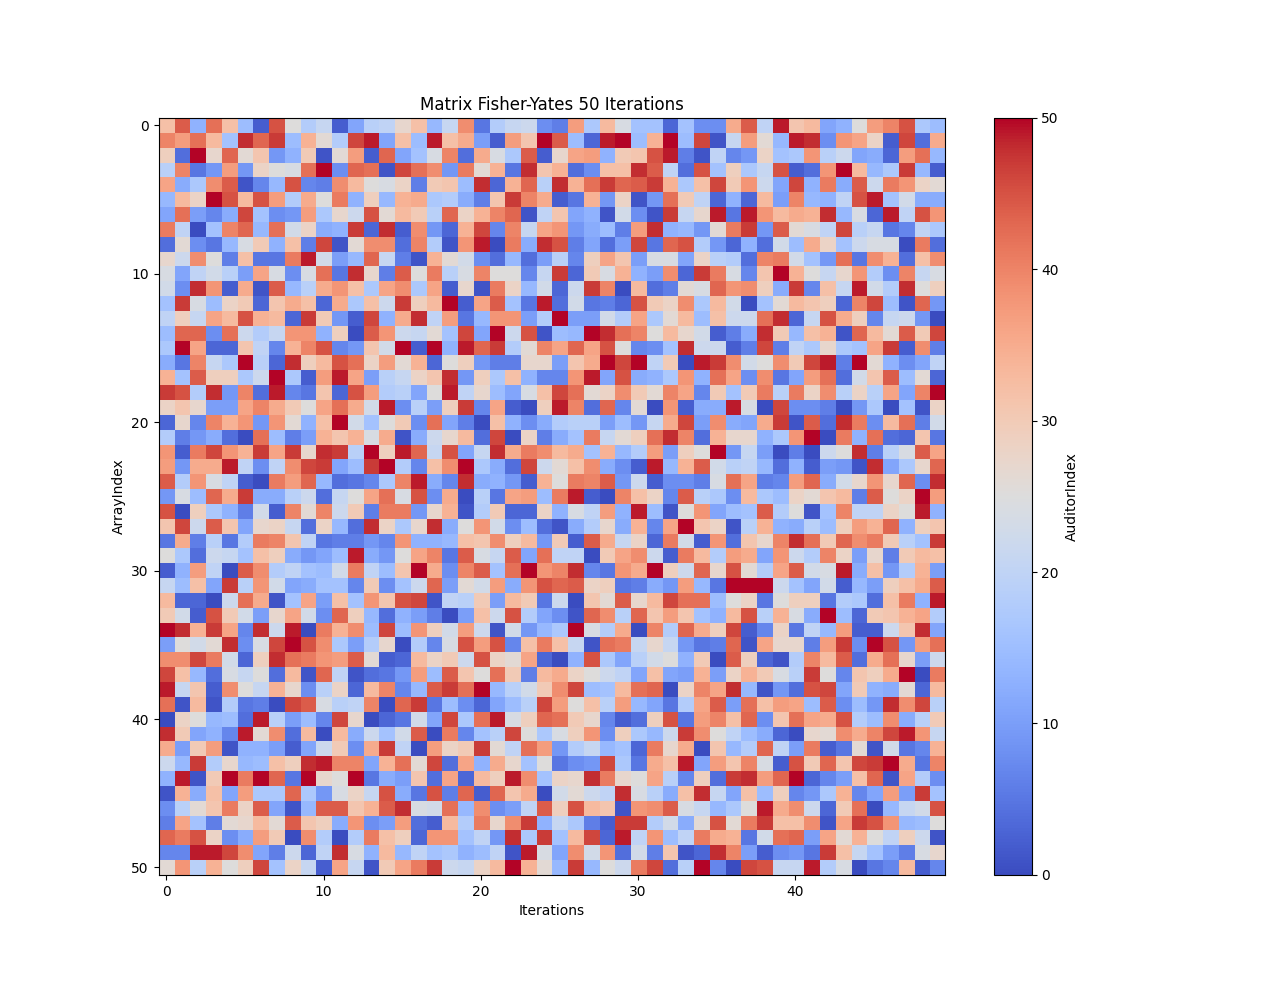
\includegraphics[width=0.99\textwidth]{matrix.png}
  \caption{Permutations
  }
  \label{fig:matrix}
\end{figure}

\begin{tcolorbox}[title=Javascript Code]
\begin{verbatim}

function shuffleAuditorPool(array) { 
  let m = array.length;
  let temp;
  let random;

  while (m) {
    random = Math.floor(Math.random() * m--);
    temp = array[m];
    array[m] = array[random];
    array[random] = temp;
  }
  
  return array;
}
\end{verbatim}
\end{tcolorbox}

The same example of Fisher-Yates with 50 iterations over a list of 50 indices but using haskell code.

\begin{figure}[ht]
  \centering
  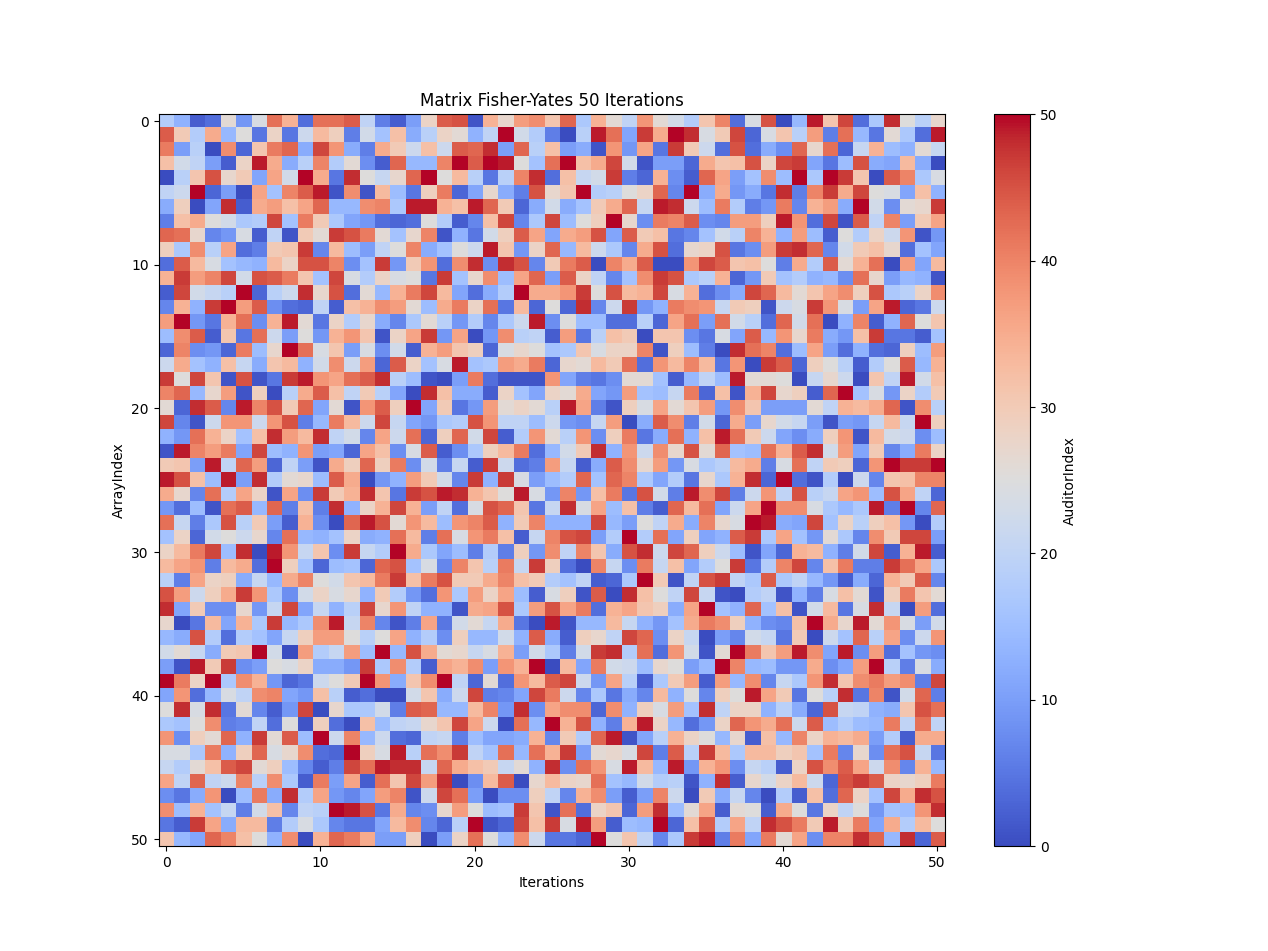
\includegraphics[width=1\textwidth]{haskell-matrix.png}
  \caption{Haskell
  }
  \label{fig:haskell-matrix}
\end{figure}


\begin{tcolorbox}[title=Haskell Code]
\begin{verbatim}

{-# LANGUAGE OverloadedStrings #-}
import System.Random (randomRIO)


shuffle :: [Int] -> IO [Int]
shuffle [] = return []
shuffle xs = do
  let m = length xs - 1
  random <- randomRIO (0, m)
  let (left, (chosen:right)) = splitAt random xs
  shuffledRight <- shuffle (left ++ right)
  return (chosen : shuffledRight)


\end{verbatim}
\end{tcolorbox}


This Fisher-Yates haskell version can be used as a reference to create a plutus implementation. The code inside a plutus contract is deterministic it is necessary to use an oracle that generates a random number for the \emph { random } variable.

\subsection { Report Minting }

The auditor report and its respective review are two different but necessarily related resources they make up a complete audit report. To ensure the immutability of its content it is necessary mint them as non-fungible assets. This can be done automatically from the backend integration at the end of the \emph{Auditing} stage. 
The latest version of the .json documents sent by the auditor and the reviewer will be hashed to subsequently mint 3 copies, 1 NFT will be sent to the wallet provided by the auditor, another will be sent to the reviewer's wallet and another will be stored in a wallet of the DAO. They will be stored in IFPS and Github.

This mechanism can be implemented in the smart contract for its operation during the \emph{Auditing} stage. For example, supplying the contract with the list of wallets that have authorization to mint and some status variables to indicate if they have already minted their report or not. However, this will be the subject of investigation for future versions of the smart contract.
\end{document}
